% !TeX root = ../main.tex

\chapter{实验结果与分析}
实验的主要目的是为了解决以下的问题:

(1) 学到的角色是否能够动态地变化,并且这种变化是为了适应环境?(章节~\ref{sec:dynamic-role})

(2) 本框架能否促进子任务的分化、专业化?即拥有相似任务的智能体在角色空间有相似的角色表征,但是有不同的子任务的智能体有不同的角色,并且这个角色在角色空间相差很远。(章节~\ref{sec:role-evolution})

(3) 这样的子任务分化能否提高多智能体强化学习的性能?(章节~\ref{sec:baseline-ablation})

(4) 角色在训练的过程中是怎样演化的?以及这种演化对性能的影响是怎样?(章节~\ref{sec:role-evolution})

本相关实验的视频能在网站上看到\footnote{\url{https://sites.google.com/view/romarl/}}。项目的代码已公开\footnote{\url{https://github.com/drdh/pymarl}}

\section{基准实验和消融实验}\label{sec:baseline-ablation}

\begin{table}[htb]
    \centering\small
    \caption{基准实验和消融实验算法}
    \label{tab:baselines}
    \begin{tabular}{cll}
      \toprule
        & 算法   & 描述                         \\
      \midrule
          & IQL   & Independent Q-learning \\
          & COMA  & Foerster et~al.~\cite{foerster2018counterfactual} \\
      相关  & QMIX  & Rashid et~al.~\cite{rashid2018qmix} \\
      算法  & QTRAN & Son et~al.~\cite{son2019qtran} \\
          & MAVEN & Mahajan et~al.~\cite{mahajan2019maven} \\
      \midrule 
             & ROMA-RAW & 无损失函数$\mathcal{L}_I$和$\mathcal{L}_D$ \\
      消融-A    & QMIX-NPS & 每个智能体都有单独的局部效用网络的QMIX \\
            & QMIX-LAR & 带有和ROMA相当数量参数的QMIX \\
       \midrule
            & $\mathcal{L}_{TD}$ & 仅有TD损失函数,同ROMA-RAW \\
      消融-B & $\mathcal{L}_{TD}+\mathcal{L}_I$ & 没有$\mathcal{L}_D$的ROMA \\
            & $\mathcal{L}_{TD}+\mathcal{L}_D$ & 没有$\mathcal{L}_I$的ROMA \\
      \bottomrule
    \end{tabular}
  \end{table}

  本实验采用的基准实验和消融实验如表~\ref{tab:baselines}所示,ROMA(Role-Oriented MARL)代指本项目算法。其中,相关算法(见图~\ref{fig:performance-baselines})是为了明确比较本算法和其他已有的算法的性能,可以看到本算法有相当优异的性能;消融-A实验中(见图~\ref{fig:performance-ablations-A}),ROMA-RAW是为了明确上一章所介绍的损失函数的有效性;QMIX-NPS是为了说明独立的效用函数并不能达到本项目算法的性能;QMIX-LAR是为了说明更多的参数不是本算法性能提升的主要原因;消融-B实验见图~\ref{fig:performance-ablations-B})是为了明确各个损失函数对性能的影响。

\begin{figure*}
    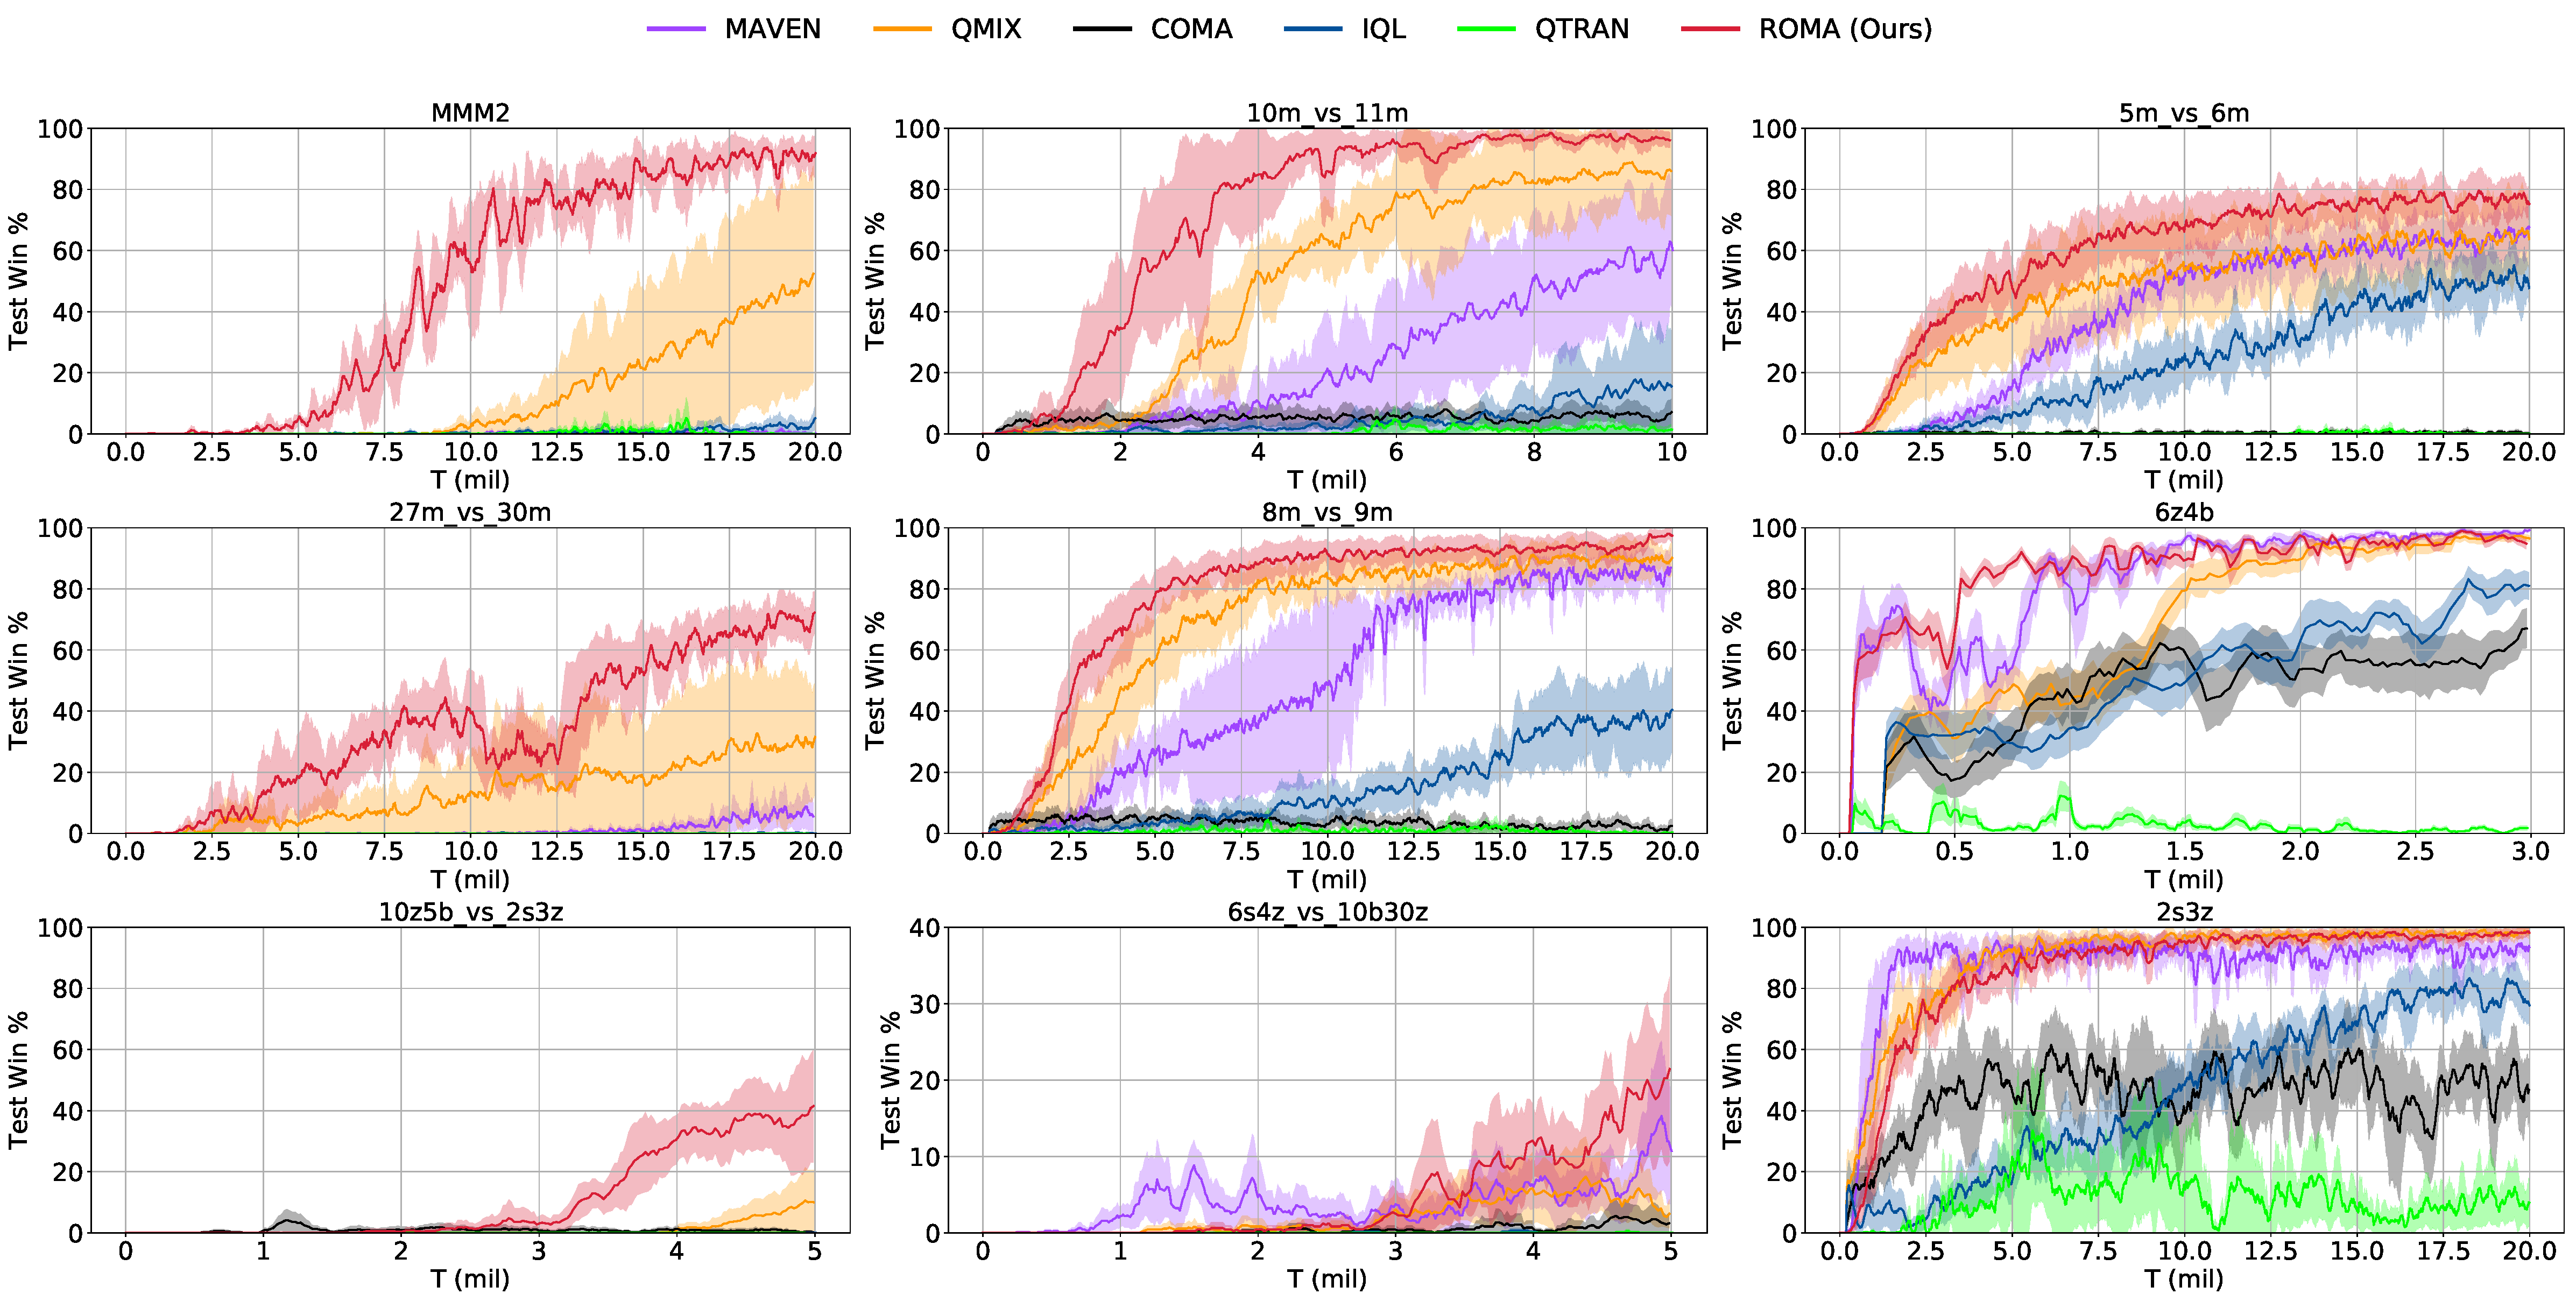
\includegraphics[width=\linewidth]{figures/learning-curve/learning_curve.pdf}
    \caption{ROMA与相关算法的性能对比}\label{fig:performance-baselines}
\end{figure*}

\begin{figure*}
    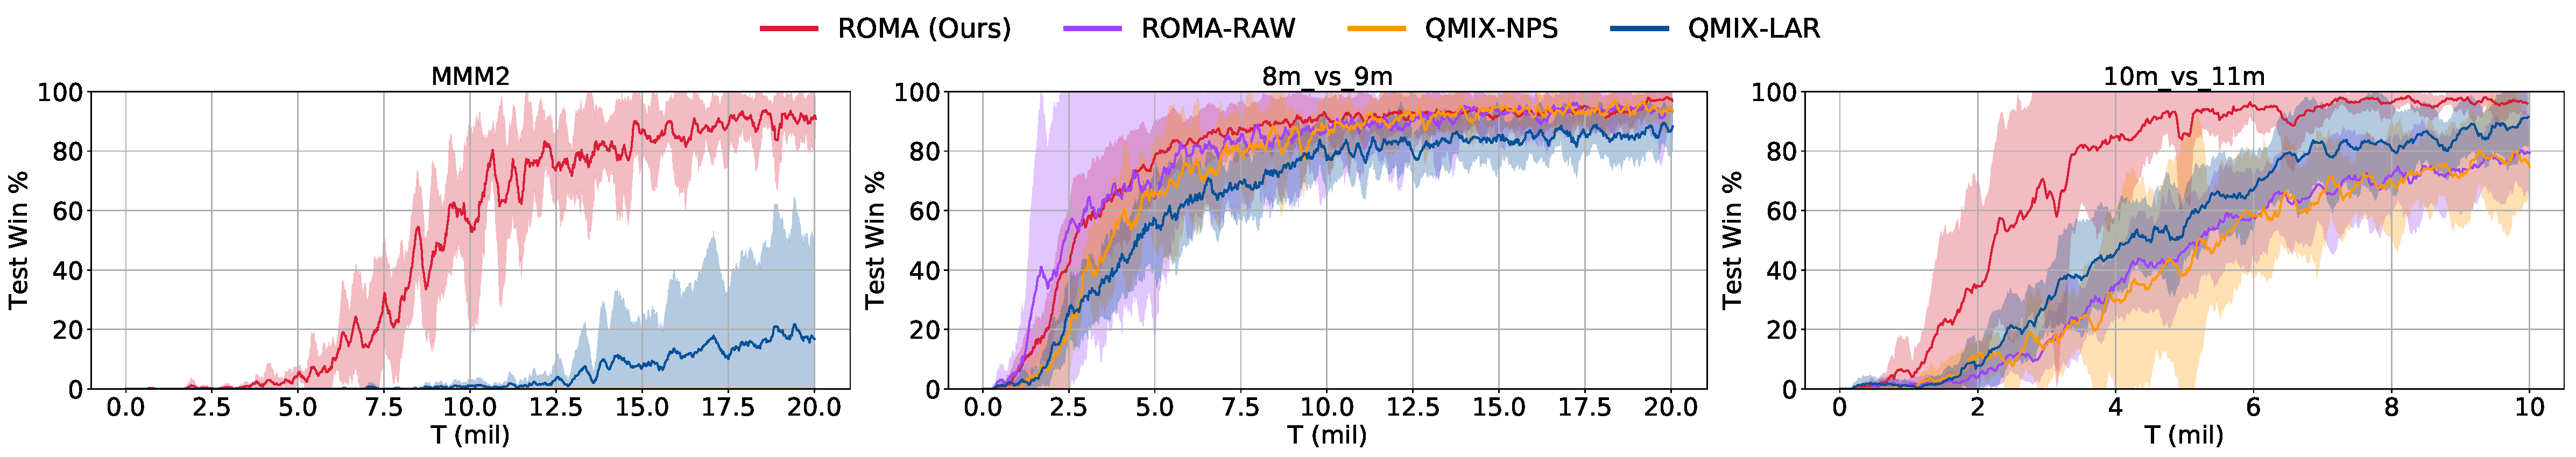
\includegraphics[width=\linewidth]{figures/learning-curve/ablation-A.pdf}
    \caption{消融实验-A}\label{fig:performance-ablations-A}
\end{figure*}

\begin{figure*}
    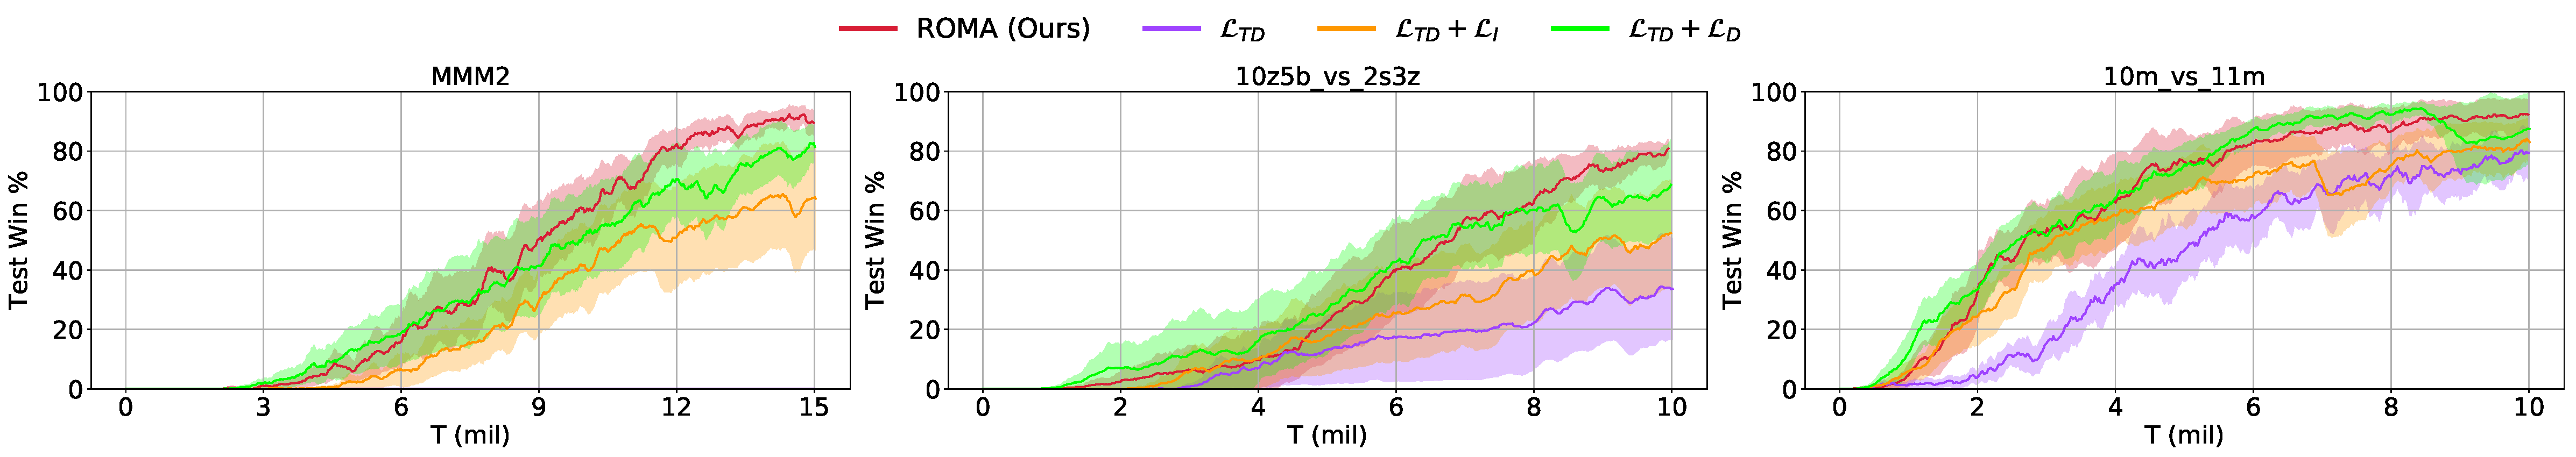
\includegraphics[width=\linewidth]{figures/learning-curve/ablation-B.pdf}
    \caption{消融实验-B}\label{fig:performance-ablations-B}
\end{figure*}
  
\section{角色的动态变化}\label{sec:dynamic-role}

\begin{figure*}
    \centering
    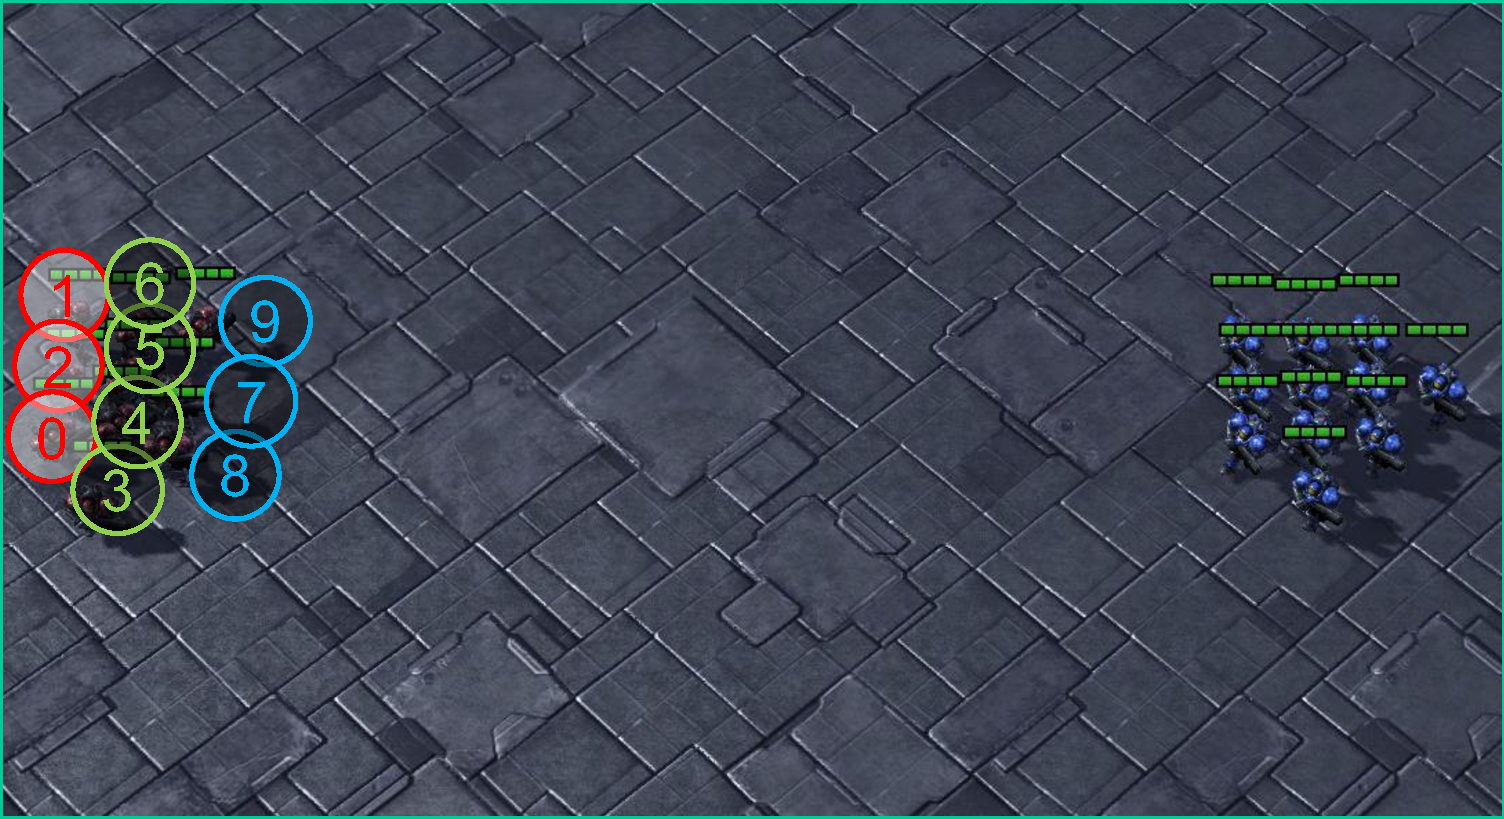
\includegraphics[height=0.24\linewidth]{figures/dynamic/10m_vs_11m-g1.pdf}\hfill
    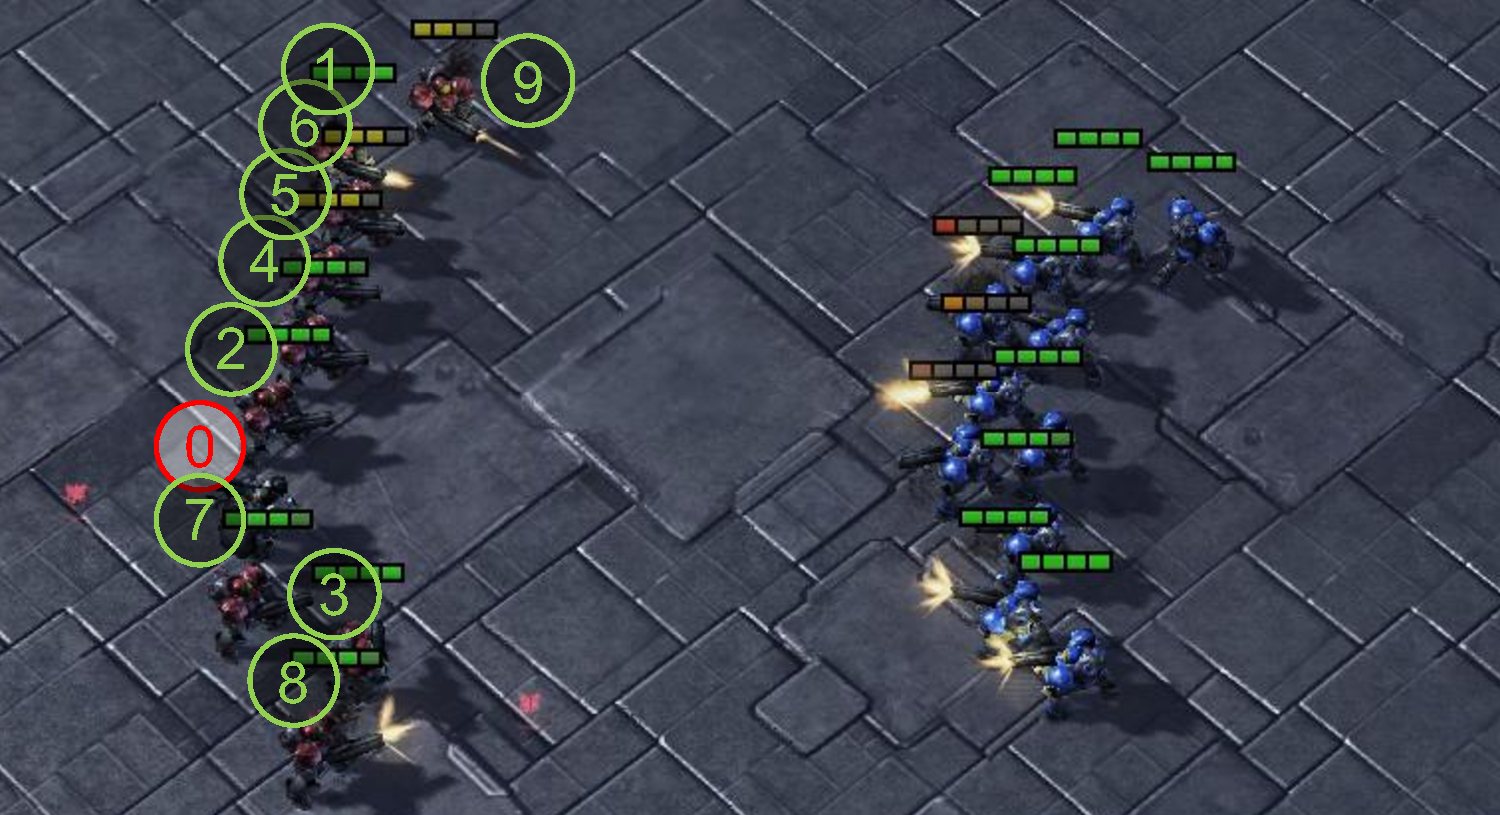
\includegraphics[height=0.24\linewidth]{figures/dynamic/10m_vs_11m-g2.pdf}\\
    \subfigure[$t$=$1$, 角色的特征是智能体的位置]{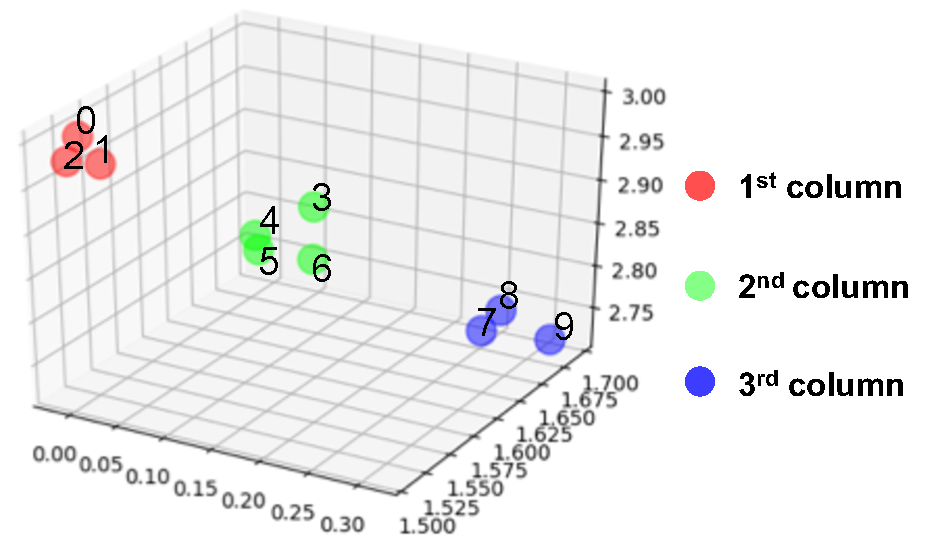
\includegraphics[width=0.48\linewidth]{figures/dynamic/10m_vs_11m-r1.pdf}}\hfill
    \subfigure[$t$=$8$, 角色的特征是智能体的血量]{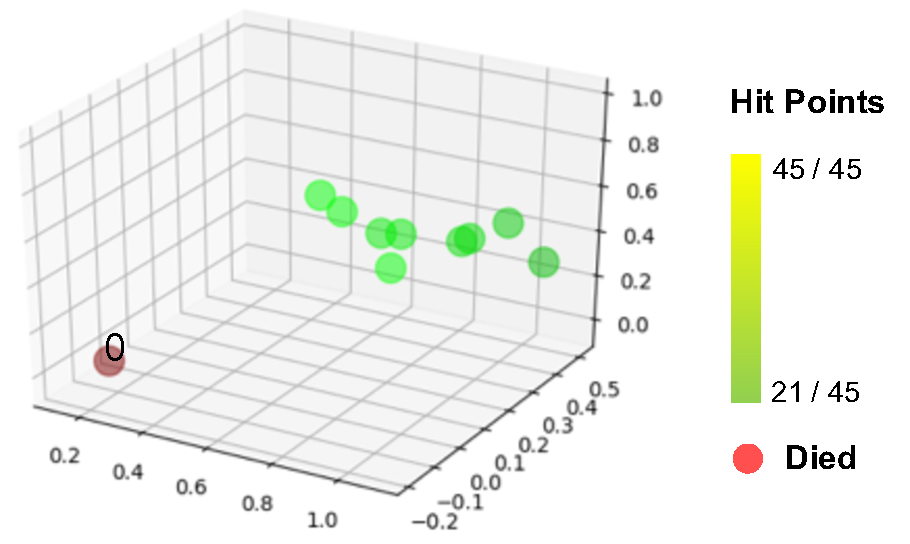
\includegraphics[width=0.48\linewidth]{figures/dynamic/10m_vs_11m-r2.pdf}}\\

    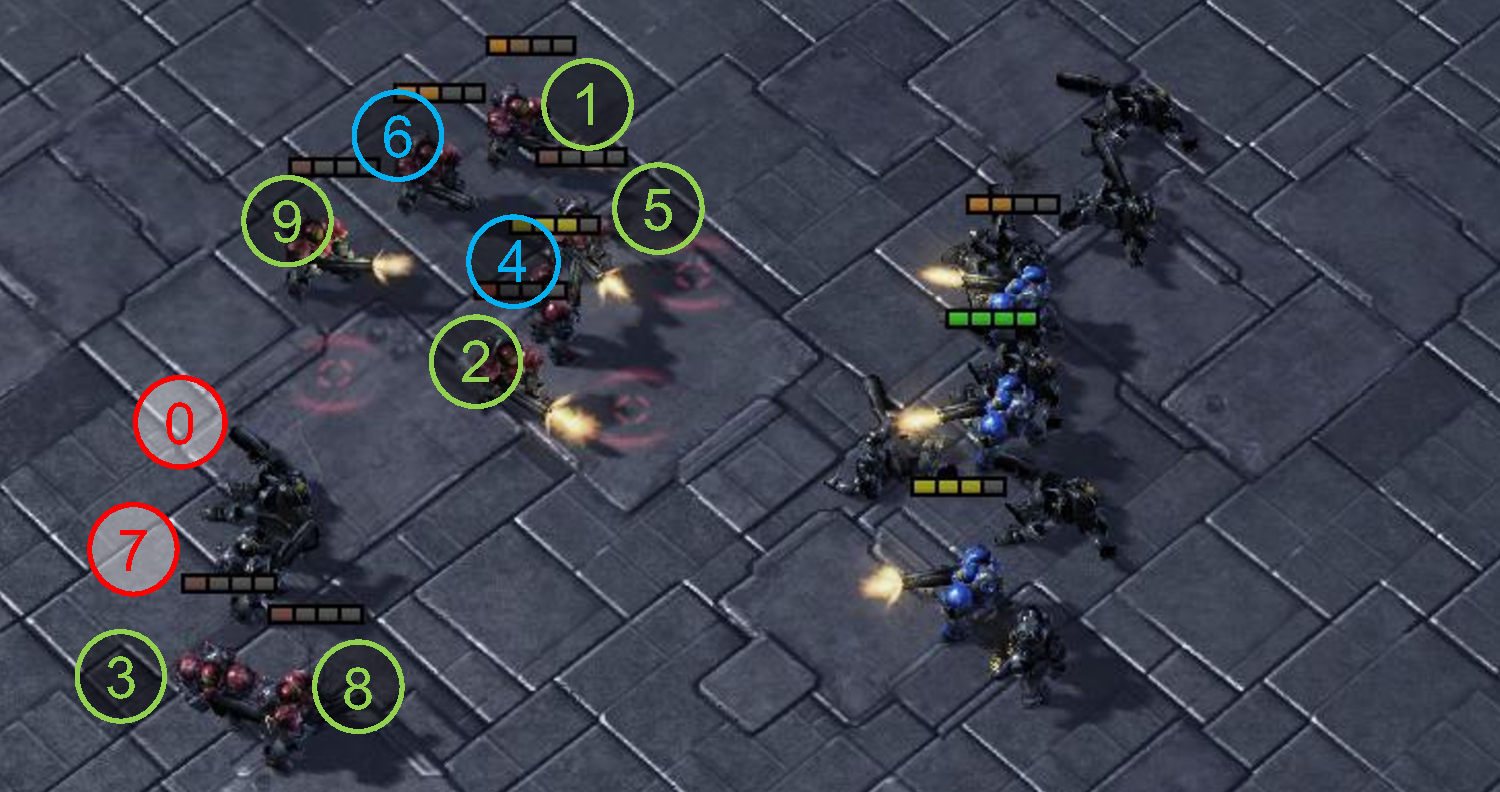
\includegraphics[height=0.24\linewidth]{figures/dynamic/10m_vs_11m-g3.pdf}\hfill
    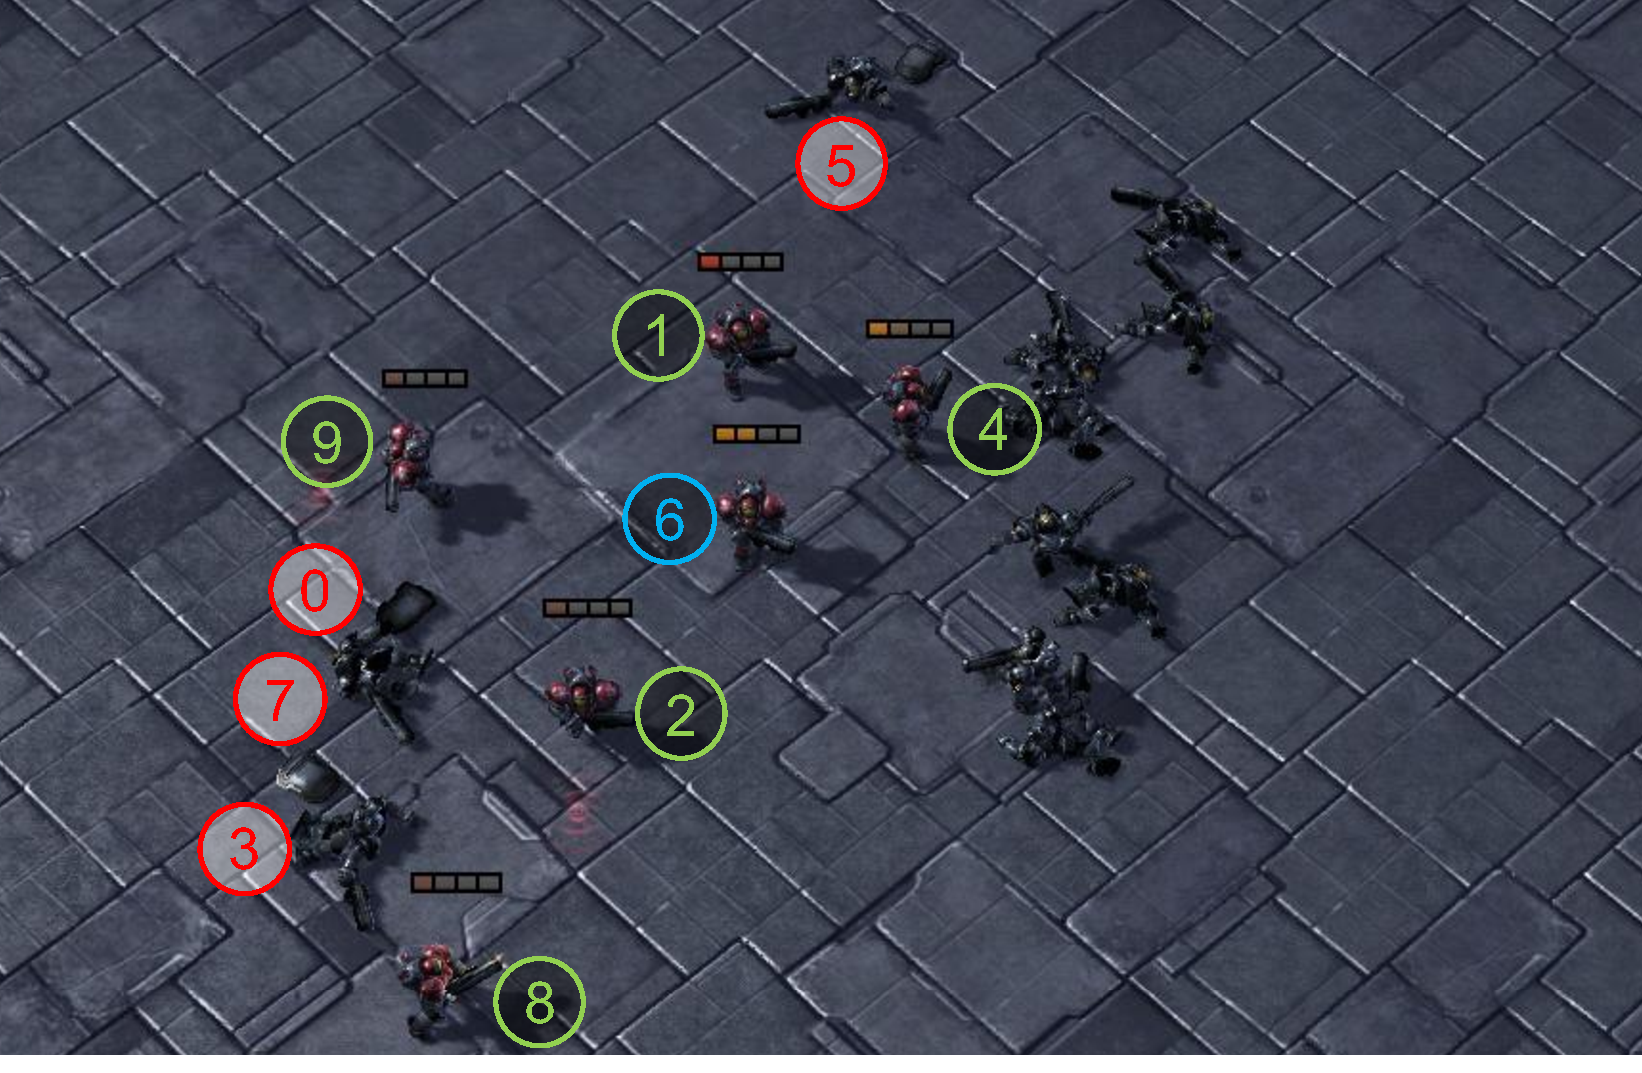
\includegraphics[height=0.24\linewidth]{figures/dynamic/10m_vs_11m-g4.pdf}\\ 
    \subfigure[$t$=$19$, 角色的特征是智能体是否存活及血量]{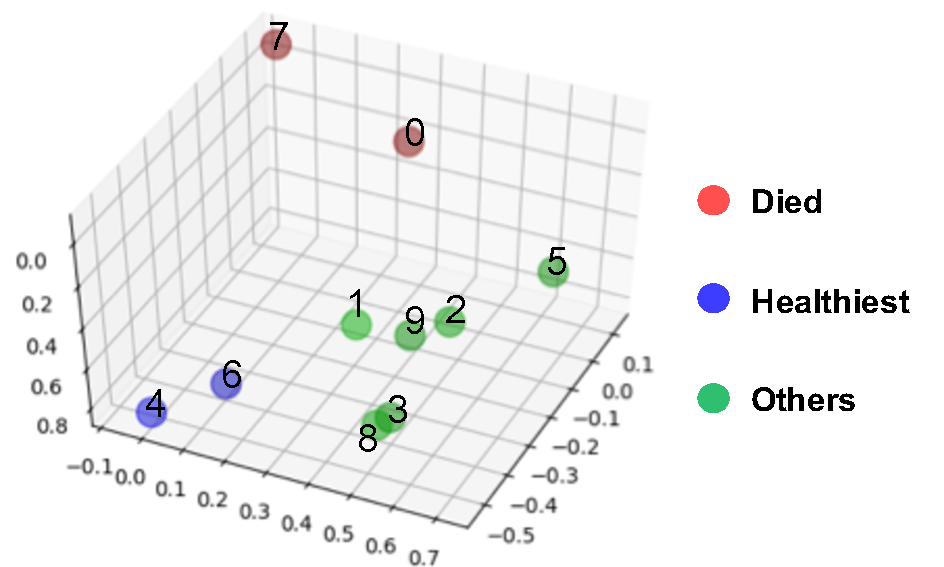
\includegraphics[width=0.48\linewidth]{figures/dynamic/10m_vs_11m-r3.pdf}}\hfill
    \subfigure[$t$=$27$, 角色的特征是智能体是否存活及血量]{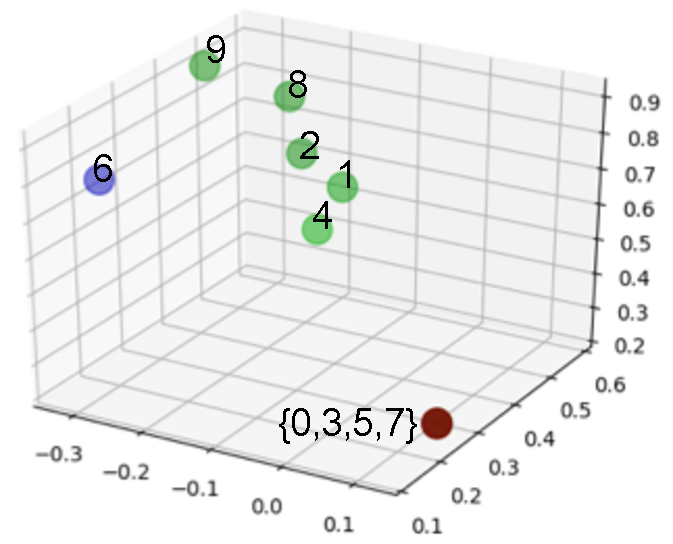
\includegraphics[width=0.32\linewidth]{figures/dynamic/10m_vs_11m-r4.pdf}}
    \caption{在一局里角色的动态变化}\label{fig:dynamic_role-10m_vs_11m}
\end{figure*}



\section{角色的表征分析}\label{sec:role-representation}

\section{角色的演化与涌现}\label{sec:role-evolution}

\section{实验配置细节}\label{sec:exp-detail}

\section{本章小结}

